\documentclass[12pt,a4paper]{article}
\usepackage[marginparsep=8pt,left=2.5cm,right=2.5cm,top=2.5cm,bottom=3cm]{geometry}
\usepackage{graphicx}% http://ctan.org/pkg/graphicx
\usepackage{titlesec}
\usepackage{xcolor}
\usepackage{xevlna}

\usepackage[utf8]{inputenc}
\usepackage[T1]{fontenc}
\usepackage{fontspec}

\setmainfont[ExternalLocation=Fonts/]{Calluna-Regular.otf}[
  BoldFont=Calluna-Bold.otf,
  ItalicFont=Calluna-It.otf,
  BoldItalicFont=Calluna-BoldIt.otf
]

\setlength{\parindent}{0pt}% Remove paragraph indent



\begin{document}
\pagenumbering{gobble}

\titleformat{\subsection}
   {\color{black}\normalfont\fontsize{17}{18}\bfseries}{\thesection}{1em}{}

%\titlespacing*{\subsection}{0cm}{0.6cm}{-0.2cm}


\center{\textbf{\fontsize{25}{30}\selectfont R-tree}}
\center{{\fontsize{14}{30}\selectfont Pavel Jahoda}}
\center{{\fontsize{12}{30}\selectfont \today}}\\[1.5cm]
%\title{\Huge R-tree}
%\author{\large Pavel Jahoda}
%\date{\normalsize \today}
%\maketitle

\flushleft\subsection*{Popis Projektu}
%\setlength{\parindent}{20pt}% Remove paragraph indent
Cílem projektu je vytvoření vlastní perzistentní implementace R-stromu, což je stromová struktura pro vyhledávání n-dimenzionálních objektů často využívaná v geografických informačních systémech. Řešení překonává požadavky zadání a kromě dotazů nad databází 2D nebo 3D objektů, zvládá i požadavky na n-dimenzionální objekty. Dotazovat se lze jak na nejbližší prvek, tak na rozsahové dotazy (tj. které objekty jsou K jednotek daleko od bodu X).  Aplikace obsahuje testovací modul, který si dokáže generovat náhodná data tak i pracovat s ručně zadanými daty. Testovací modul kontroluje vyváženost stromu, korektnost velikosti bounding boxů, také testuje dotazování na nejbližšího souseda a rozsahové dotazy. \\[0.6cm]
Navíc oproti zadání, které umožňuje generování náhodných dat (které generuji v testovacím modulu), stahuji data z aplikace flightradar od která s 5 minutovým zpožděním získávám data o letištích a také letadlech, která jsou v daný moment ve vzduchu. Kromě polohy získávám rychlost, typ letadla, leteckou společnost ke které letadlo patří a další zajímavé údaje. Kromě náhodných dat je tedy možné se dotazovat i na letecká data.  \par \bigskip

\subsection*{Způsob řešení}
V této sekci se především zaměřím na popis vkládání prvku z čehož je pochopitelný celý princip algoritmu. Když chceme vložit prvek do stromu nacházíme se nejprve v kořeni stromu (root). Pokud má kořen jako potomky listy, stane se náš prvek potomkem kořene. Pokud nemá kořen listy zjistíme kolika potomkům by se při vkládání našeho prvku nemusel zvětšovat minimal bounding box (prvek je uvnitř bounding boxu). Pokud je takových potomků více než jeden, vnoříme se do toho, který má střed minimal bounding boxu nejblíž našemu vkládánému prvku. V případě že je takový potomek jeden vnoříme se do něj a pokud takový potomek neexistuje, vnoříme se do potomka, kterému by se objem minimal bounding boxu zvětšil po přidání prvku nejméně. Takhle se budeme vnořovat dokud nedojdeme do uzlu který obsahuje listy a do něj prvek vložíme\\[0.6cm]

Při vkládání prvku do uzlu se může stát, že uzel obsahuje maximum námi nastaveného počtu potomků, v takové případě dochází na dělení uzlů. Z jednoho uzlu s 4 potomky a 1 vkládaným prvkem se může teoreticky stát 2 nové uzly, kde jeden má 2 potomky a druhý 3 potomky. Jeden z nových uzlů se posunul na místo předchozího starého uzlu a druhý uzel se stává "prvkem" vkládaným do předka našeho starého uzlu. Takovým způsobem se můžeme dostat až do kořenového uzlu, kde kořen rozdělíme na dva nové uzly jejichž předkem se stane úplně nový kořen.\\[0.6cm]

V aplikaci je možné použít tři různé algoritmy na dělení uzlu. První algoritmus je náhodný, který zajistí pouze to, že nové uzly budou mít splněné podmínky na minimální a maximální počet potomků. Druhým algoritmem je řešení hrubou silou. Toto řešení prochází všechny validní permutace rozdělení uzlu a vybere takové, které vytvoří uzly s nejmenším součtem objemů minimal bounding boxů. Třetí řešení je variace\cite{nodeSplitting} na quadratic split. Stejně jako v quadratic split algoritmu se nejprve vyberou dva prvky které není mít výhodné ve stejném uzlu a ty budou prvními prvky nových uzlů. První z vybraných dvou prvků bude mít nejmenší součet souřadnic a druhý prvek naopak největší součet souřadnic, takový výběr prvků není optimální, nicméně je jeho asymptotická složitost pouze O(N) narozdíl od algoritmu Quadratic split, který má časovou asymptotickou složitost výběru prvních dvou prvků $O(N^2)$\cite{original}. Zbytek prvků se přerozdělí tak, že se vybere m-1 (kde m je minimální počet potomků uzlu) prvků které jsou nejblíže k prvnímu vybranému prvku a přidají se do uzlu společně s ním. Stejně se vybere m-1 prvků k druhému prvku a zbytek se rozdělí podle toho, jestli je daný prvek blíž k prvnímu nebo druhému prvku.\\[0.6cm]

Algoritmus na hledání nejbližšího prvku v R-stromu funguje následovně\cite{queries}. Pokud jsme uzlu co má listy, zjistíme jestli některý z listů není blíž než dosavadní nejbližší prvek a popřípadě dosavadní nejbližší prvek přepíšeme. Pokud nejsem v uzlu co má listy, jsme v uzlu co má potomky s bounding boxy. Tyto potomky seřadíme podle vzdálenosti minimal bounding boxu od dotazovaného prvku a vnoříme se do těch které mají zmíněnou vzdálenost menší než vzdálenost dosavadního prvku s nejmenší vzdáleností. Rozsahový dotaz funguje na obdobném principu. 
\par \bigskip

\subsection*{Implementace}
Projekt byl programovaný v jazyce Python3. Na grafické výstupy byla použita knihovna plotly (pip3 install plotly) a flightradar24 (pip3 install flightradar24) (na letecká data). Na znázornění grafů v experimentální sekci byla použita knihovna matplotlib. Pro grafické výstupy se spouští třída main (python3 src/main.py). Samotný R-strom lze testovat pouze s nainstalovaným jazykem Python3 voláním třídy RTreeTestCases (python3 src/RTreeTestCases.py).\par \bigskip

\subsection*{Příklad výstupu} \par \bigskip
\begin{center}
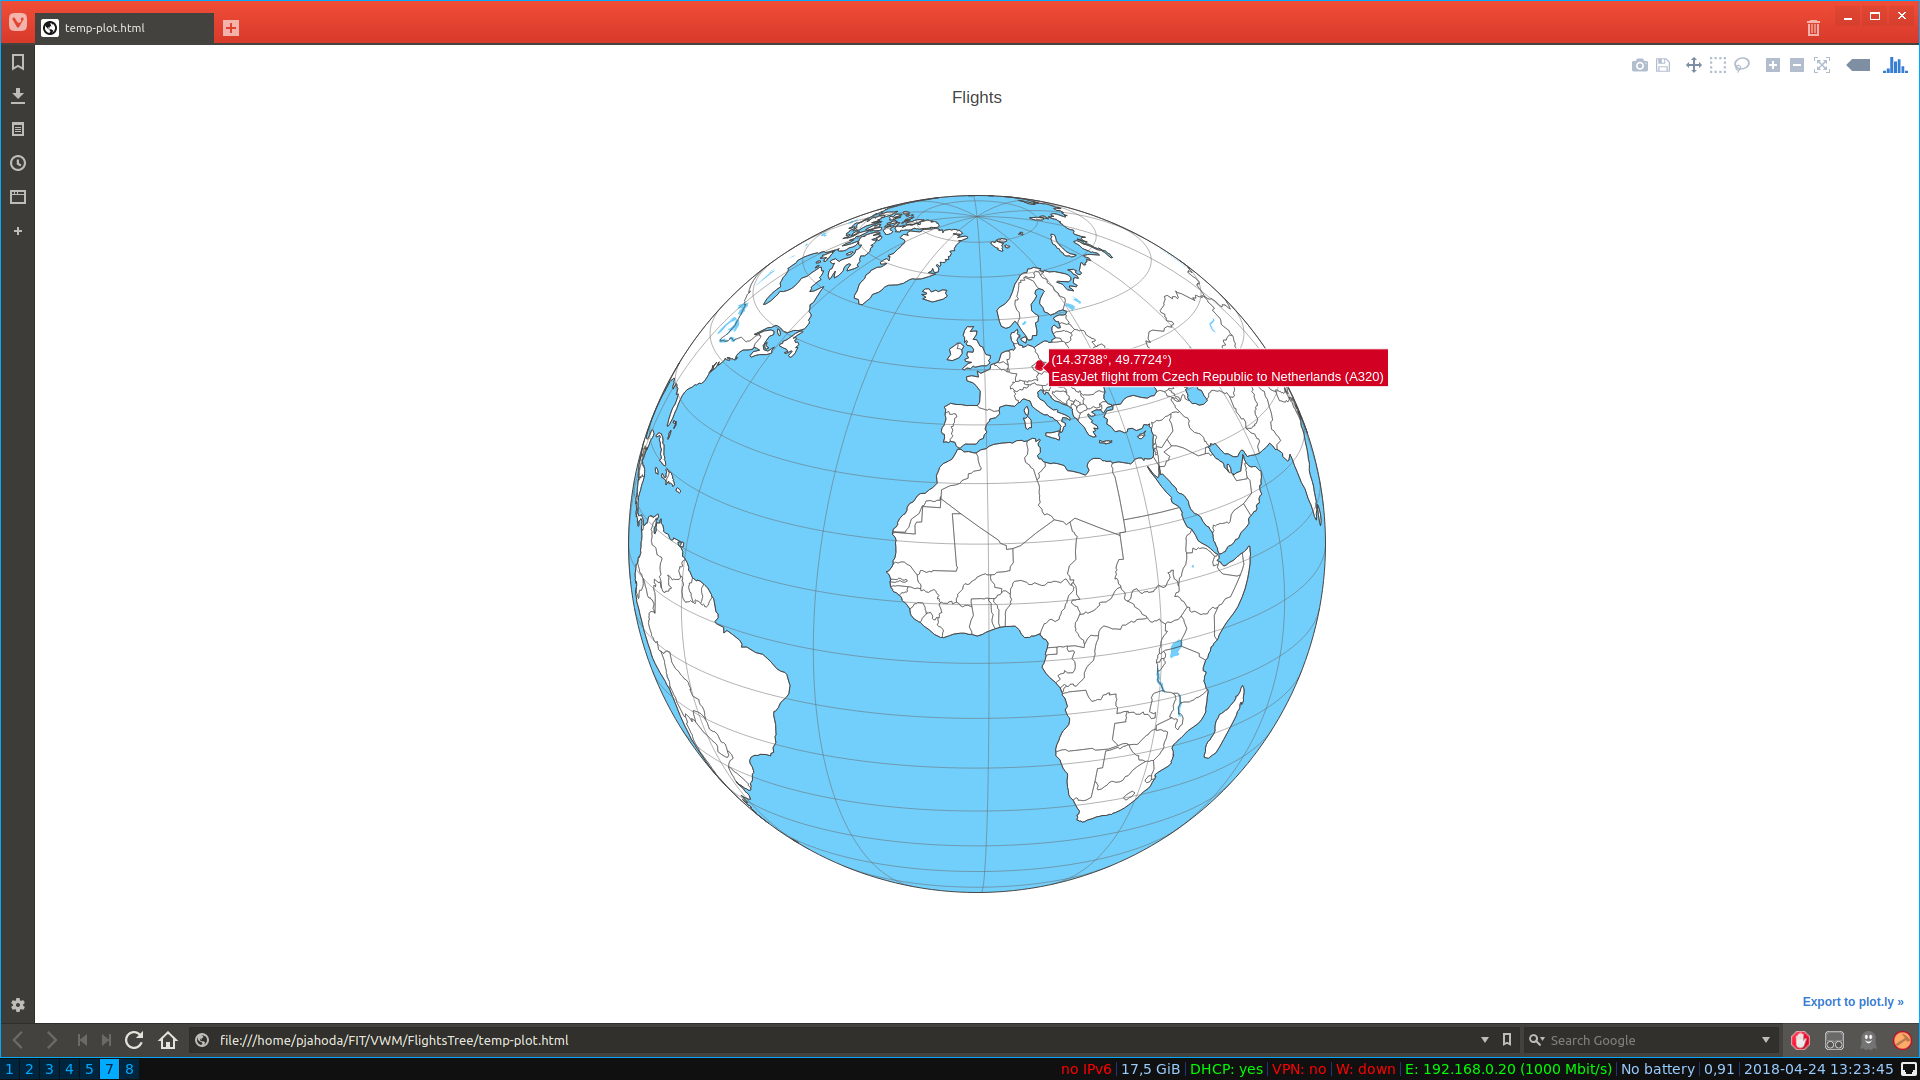
\includegraphics[width=15cm, height=8cm]{output1}
\end{center}
Jak je patrné na obrázku výše jedná se o webové grafické rozhraní. Obrázek ukazuje výstup rozsahového dotazu na okolí Prahy.

\begin{center}
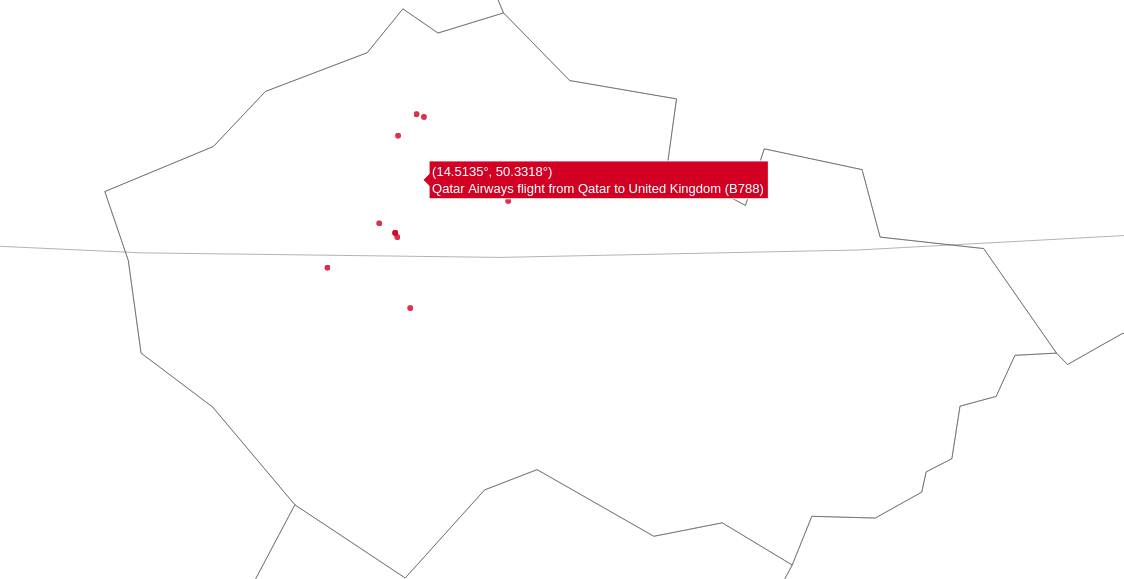
\includegraphics[width=15cm, height=8cm]{output2}
\end{center}
Zde je přiblížený výstup k předchozímu dotazu. V obrázku je vidět, že aplikace ukazuje ke každému nalezenému letadlu odkud kam letí a k jaké letecké společnosti patří.

\begin{center}
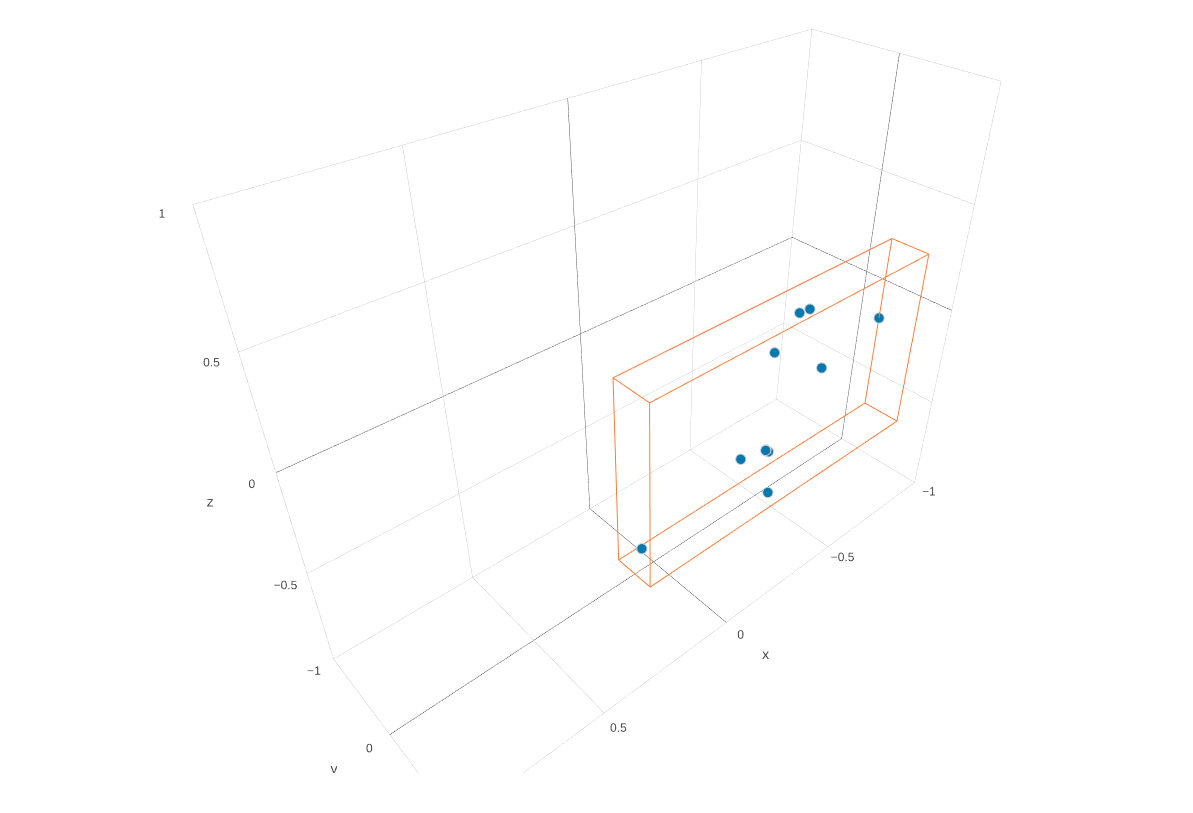
\includegraphics[width=15cm, height=8cm]{output3}
\end{center}
Výstup je také možné zobrazit ve 3D prostoru.


\subsection*{Experimentální Sekce}
R-strom nabízí hned několik věcí na testování. Z hlediska rychlost vkládání prvků a následných dotazů můžeme porovnávat vliv různých metod dělení uzlů, počet potomků uzlu, počet dimenzí nebo vzdálenost u rozsahového dotazu.\\[0.5cm]
Tabulka níže (Table 1) ukazuje vliv volby metody dělení uzlů (když uzel dosáhl maximálního množství potomků) na rychlost vkládání prvků a rychlost rozsahových dotazů. Data v tabulce jsou zprůměrovaná z pěti různých testování na stromu s maximálním množstvím 8 potomků na uzel, na trojdimenzionálních datech na 2 000 datech a 20 000 dotazech. Data jsou v sekundách.
 
\begin{table}[ht]
\begin{center}
\caption{Rychlost vkládání a dotazů}
\label{tbl:bins} % spaces are big no-no withing labels
\begin{tabular}{|c|cc|} 
\hline
\multicolumn{1}{|c}{} & \multicolumn{1}{c}{Insert} & \multicolumn{1}{c|}{Query} \\
\hline
Random & 1.0669 &   19.45292 \\
\hline
Brute force & 4.73896 &   5.33882 \\
\hline
Heuristic & 0.91115 &   7.51662 \\
\hline
\end{tabular}
\end{center}
\end{table}

Výsledek je očekávaný. Metoda hrubou silou (brute force) je jasně nejpomalejší pří vkládání, zatímco na dotazech vyhrává. Metoda dělení heuristikou nejenže nejrychleji vkládá prvky, ale vede si obstojně i v rozsahových dotazech, což je důvodem proč jsou heuristiky na R-stromech používané. Na druhou stranu metoda náhodného rozdělení uzlů je suverénně nejhorší na rozsahové dotazy.\\[0.5cm]
Na grafu níže můžeme pozorovat vliv počtu potomků uzlu na dobu vkládání prvků. Zatímco vkládání s dělením uzlu heuristikou nebo náhodným dělením je s vzrůstajícím počtem potomků dokonce nepatrně rychlejší tak u dělení hrubou silou můžeme pozorovat velký pokles rychlost přidávání. Tento fakt je způsoben tím, ze řešení hrubou silou zkouší všechny možné permutace rozdělení uzlu, což je asymptoticky exponenciální.

\begin{center}
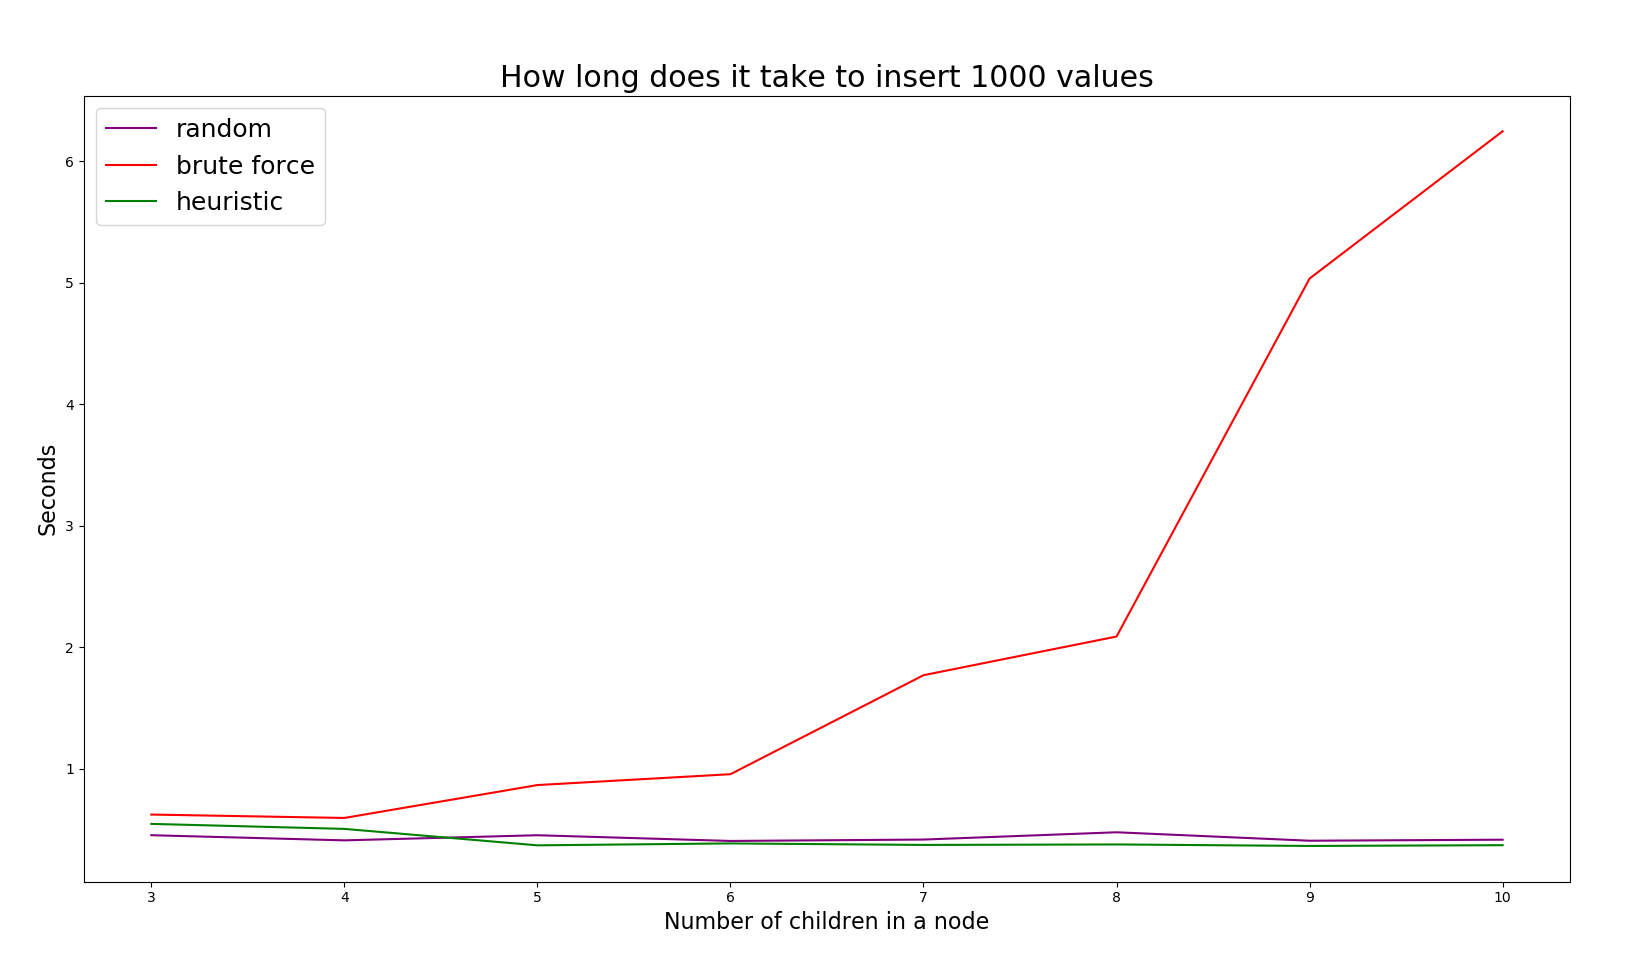
\includegraphics[width=15cm, height=8cm]{nOfChildren}
\end{center}

Na závěr experimentální sekce bych zde uvedl, že počet dimenzí hraje naprosto minimální vliv na rychlost vkládání nebo na rychlost rozsahových dotazů. Toto zjištění potvrzuje silné stránky R-stromu.

\subsection*{Diskuze}
Aplikace v momentální verzi neobsahuje plně funkční grafické uživatelské rozhraní(dále jen GUI). Momentálně se ve třídě main zavolá funkce, které se předá latitude a longitude a vzdálenost od tohoto místa a aplikace najde veškeré letadla v této oblasti. Aplikace také není plně perzistentní, nicméně šetří pamětí, tím, že každý prvek v r-stromu neobsahuje celý objekt, ale pouze souřednice a index objektu. Většina omezení, popřípadně nedokonalostí projektu byla způsobena především tím, že jsem pracoval sám na projektu určeném pro dvě osoby. Tvorba plně funkční aplikace s GUI by byla nad rámec tohoto předmětu. V grafické verzi je latitude a longitude přepočítáváno na x,y,z validním způsobem pokud by země byla perfektní koule, což není. Naštěstí tento nepřesný výpočet nezpůsobuje příliš velké odchylky, takže přestože problém existuje - není na první pohled viditelný. 

\subsection*{Závěr}
Experimenty potvrdili výhody a nevýhody různých typů dělení uzlů R-stromu. Dále také potvrdili, že R-strom si zachovává efektivitu s rostoucím počtem dimenzí objektů. Do budoucna projekt nabízí možnost rozšiřitelnosti v podobě například lepšího GUI.

%\subsection*{Reference}
\bibliographystyle{IEEEtran}
\begin{thebibliography}{9}
\bibitem{nodeSplitting} A. F. Al-Badarneh, Q. Yaseen and I. Hmeidi, \textit{A new enhancement to the
R-tree node splitting},
(Journal of Information Science, 2009)
\bibitem{original} A. Guttman \textit{R-trees. A Dynamic Index Structure
For Spatial Searching}, ACM 1984
\bibitem{queries} Roussopoulos, Nick, S. Kelley and F. Vincent. \textit{Nearest neighbor queries} 
(ACM sigmod record. Vol. 24. No. 2. ACM, 1995)
\end{thebibliography}


\end{document}
